\documentclass{article}
\usepackage{iclr2027_conference,times}
\usepackage{amsmath,amssymb,booktabs,graphicx,microtype}
\usepackage{hyperref}
\iclrfinalcopy
\title{Calibration Objectives for\\Transferred Speculative Drafters\\\large Preliminary evidence report}
\author{Anonymous Authors}
\begin{document}
\maketitle
\lhead{Working draft: experiments and manuscript incomplete}
\begin{abstract}
We investigate whether acceptance-aware token supervision improves a
transferred feature-conditioned speculative drafter. This working report
records completed development experiments from an ongoing study, rather
than a finished submission. With 4,096 training records and three epochs,
the reproduced feature objective outperformed the token-loss configurations
in the earlier development comparison. A separate 512-anchor study crosses
adapter architecture with CE and AUF; its final results are not yet available.
Additional drafter LoRA training from the feature-fitted checkpoint gives
near-parity throughput in its first full timing. Repeated timing, broader
workloads, scaling, and confirmation experiments remain unfinished.
\end{abstract}

\section{Question and controlled interventions}
RelaySpec transfers a frozen feature-conditioned drafter to a new target
through a learned linear interface. We compare the reproduced ZIP feature
objective with ordinary token cross-entropy (CE) and accept-until-fail
(AUF) cross-entropy while keeping the original targets frozen. No
target-side LoRA adaptation is used. Equal record counts and epochs do
not imply equal optimizer updates, supervised positions, or compute
across feature and token objectives.

For valid supervised positions $m_{b,j}$, draft probabilities
$p_{\theta,b,j}$, and labels $y_{b,j}$ from the original target's rollout,
the detached AUF support is
\begin{align}
 w_{b,j}&=\operatorname{stopgrad}\left[
 \prod_{i<j}\left(1-m_{b,i}+m_{b,i}
 \mathbf{1}[\arg\max_v p_{\theta,b,i}(v)=y_{b,i}]\right)\right],\\
 \mathcal L_{\mathrm{AUF}}&=-\frac{\sum_{b,j}m_{b,j}w_{b,j}
 \log p_{\theta,b,j}(y_{b,j})}{\sum_{b,j}m_{b,j}w_{b,j}}.
\end{align}
The clean anchor and padding are excluded. The first incorrect proposal
remains supervised; positions after it do not. Normalization is performed
inside each microbatch, followed by equal microbatch averaging per update.
Pure AUF is used for this token intervention; no simultaneous MSE or KL
term is added. ZIP denotes the reproduced layer and normalized fused-context
feature objective, with its original position sampling and example weighting.

\section{Earlier development evidence}
Each result below uses 128 Numina development requests, a maximum of
2,048 generated tokens with natural EOS, fitting seed42, and one warmed
timing. The inference backend is vLLM0.28.0 on L40S hardware. These are
development measurements, not untouched confirmation results. Exactness
means equality of the complete generated token sequence with the paired
autoregressive (AR) output. It does not establish mathematical correctness
of an answer or a universal guarantee across numerical configurations.

\begin{table}[h]
\centering\small
\begin{tabular}{llrrr}
\toprule
Target & Objective & Tokens/s & Speedup & Exact/128 \\
\midrule
Qwen3-8B & AR & 24.56 & 1.00 & reference \\
 & ZIP & 173.94 & 7.08 & 128 \\
 & CE & 108.75 & 4.43 & 128 \\
 & AUF & 98.81 & 4.02 & 128 \\
\midrule
Llama-3.2-3B & AR & 46.01 & 1.00 & reference \\
 & ZIP & 186.93 & 4.06 & 128 \\
 & CE & 142.23 & 3.09 & 128 \\
 & AUF & 112.86 & 2.45 & 128 \\
\bottomrule
\end{tabular}

\caption{Completed loss replacements. Qwen3-4B and Llama-3.1-8B drafters
serve the listed targets. Speedup is relative to each target's own AR
run. Differences in target and runtime configuration preclude interpreting
cross-family absolute throughput as a model ranking.}
\end{table}

\begin{figure}[t]
\centering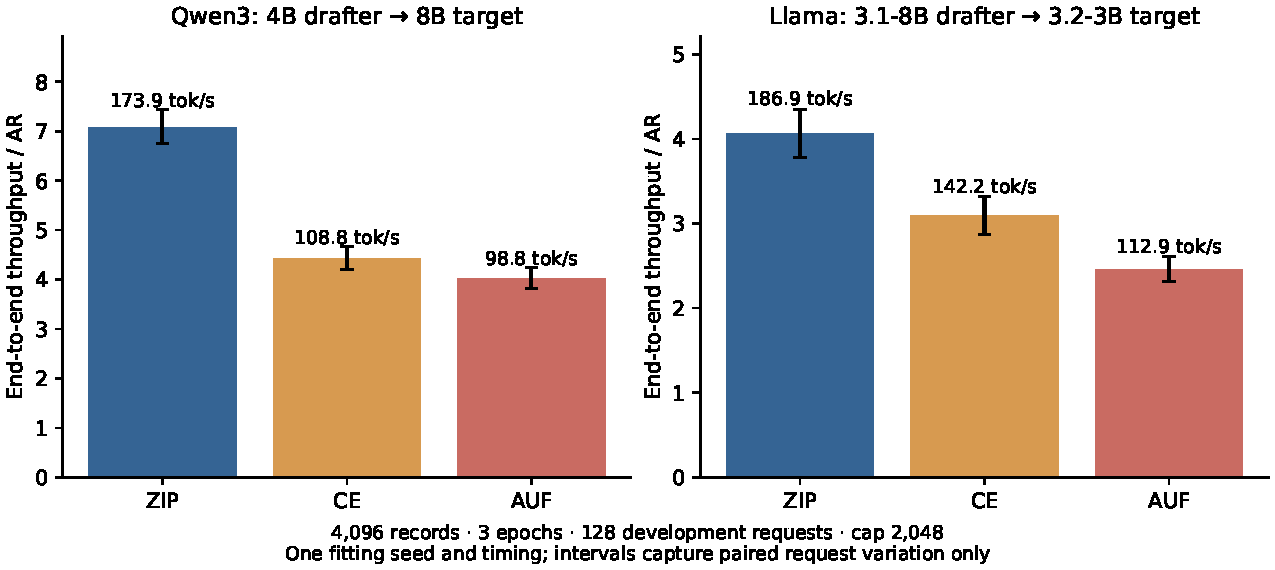
\includegraphics[width=\linewidth]{figures/objectives.pdf}
\caption{Throughput after fitting each objective. Intervals use 10,000
paired request bootstrap samples; they exclude fitting-seed, timing-order
and selection uncertainty. The current AUF intervention reduces throughput
relative to feature fitting in both completed settings.}
\end{figure}

\section{Does adapting the drafter add value?}
We additionally hold the trained ZIP interface fixed and adapt drafter
attention and MLP projections with rank32 LoRA, using either CE or AUF.
All branches reuse the same 4,096 records. The initial ZIP fit receives
three epochs and each continuation receives three additional epochs.
This is an incremental adaptation test; it is not an equal-total-compute
comparison with the unchanged ZIP checkpoint. No source transformer is
restored during decoding.

\begin{table}[h]
\centering\small
\begin{tabular}{lrrr}
\toprule
Qwen adaptation & Tokens/s & Ratio to ZIP & Exact/128 \\
\midrule
ZIP (earlier timing) & 173.94 & 1.000 & 128 \\
ZIP + drafter LoRA CE & 173.10 & 0.995 & 128 \\
ZIP + drafter LoRA AUF & 174.83 & 1.005 & 128 \\
\bottomrule
\end{tabular}

\caption{First complete drafter-LoRA timing, compared with the earlier
ZIP timing. Three fresh unchanged ZIP/native controls and repeated
LoRA timings are pending. These approximately half-percent differences
do not establish a winner.}
\end{table}
Merged-checkpoint logits agree exactly with the training implementation.
The vLLM attachment check also verifies full projection tensors and the
derived fused context-KV buffer against the exported weights. All reported
LoRA outputs match paired AR outputs on 128/128 requests.

\section{Scope and unfinished evidence}
Our reported Qwen3 experiments use a shared tokenizer and token-ID
vocabulary; the mapper adapts hidden representations or the fusion
interface, not vocabulary IDs. Consequently, these results do not
demonstrate heterogeneous-vocabulary DFlash support.

Qwen14 evaluation, multiple-workload measurements, timing and fitting-seed
replication, data and compute scaling, capacity, regularization, untouched
confirmation, and the final Transformers replications remain incomplete.
Related work, contribution claims and the full discussion will be written
against the completed evidence. This report does not claim a new
state-of-the-art method or submission readiness. Machine-readable claim
and source hashes are recorded in \texttt{claim\_evidence.json}.

\section{Controlled 512-anchor study in progress}
The new study separates initialization, architecture, and token objective.
The source-target pairs are Qwen3-4B to Qwen3-8B, Llama-3.1-8B to
Llama-3.2-3B, and Qwen3-4B to Llama-3.1-8B. Source sizes identify the
original conditioning transformer, not the much smaller DFlash drafter.
Original RelaySpec and ZIP are feature-fitting procedures, not CE losses.
Their unchanged checkpoints remain controls for CE and AUF continuations.
Interfaces include the normalized RelaySpec map, a residual fusion adapter,
five dense layer maps, one unrestricted fusion matrix, and five independent
rank-56 residual layer adapters. The source drafter and target remain frozen.

DFlash's Appendix A.1 reports 512 sampled anchors per sequence and
position-decayed CE\footnote{\url{https://arxiv.org/html/2602.06036v1}}.
Uniform CE and AUF are explicit objective interventions. Our protocol uses
4,096 cached records, a 4,096-token rollout cap, and 16,000 presentations at
global batch eight. Short records supply fewer distinct anchors. Tuning uses
a separate 32-request validation set; final comparisons require 128 requests,
a 2,048-token cap, and three timing repetitions.

\begin{table}[t]
\centering\small
\begin{tabular}{lll}
\toprule
Interface & Initialization & Trainable continuation \\
\midrule
RelaySpec interface & Original feature fit & Normalized dense map \\
Fusion residual & ZIP feature fit & One rank-56 $BA$ update \\
Five layer maps & ZIP feature fit & Five dense maps \\
Dense fusion & ZIP feature fit & One dense fusion matrix \\
Five layer residuals & ZIP feature fit & Five rank-56 $BA$ updates \\
Fresh dense control & Kaiming initialization & One dense fusion matrix \\
\bottomrule
\end{tabular}
\caption{Registered interventions, each crossed with uniform CE and AUF.
Unchanged original RelaySpec and ZIP checkpoints provide separate controls.
This is an experimental-design table, not a completed performance comparison.}
\end{table}

Each interface/loss pair screens learning rates $10^{-4}$, $3\times10^{-4}$,
and $6\times10^{-4}$ at 100 updates. The two best verified candidates advance
to 500 updates; one advances to 2,000 updates. Each budget uses a fresh fit
from its registered initializer with its own warmup/cosine schedule, rather
than treating the earlier short schedule as a prefix of the longer schedule.
Selection uses exact-output-verified validation throughput, with no selection
on the final 128 requests. CE and AUF may select different learning rates;
the final comparison therefore concerns separately tuned recipes, not a
fixed-learning-rate causal estimate of the loss alone. Three final timing
repetitions measure timing variation, not variation across training seeds.

Batched serving is a separate measurement protocol: fixed request batches of
four or eight report total generated tokens divided by total batch wall time.
Amortized per-request batch time is not individual request latency. GPU
validation and final batched comparisons remain pending. Cross-family data
assembly additionally records eligible-anchor coverage, since shared text
boundaries can further restrict the number of valid anchors below 512.

The first Qwen8 five-BA fits completed 100 updates (800 presentations) with
1,863,680 trainable parameters. AUF took 337.8 seconds and CE 339.7 seconds
on two L40S GPUs; both peaked near 17.04 GB allocated memory on rank zero.
These incremental fitting costs exclude ZIP initialization and rollouts.
Both exports passed frozen-weight and folding checks. On the separate
32-request tuning set with a 512-token cap, these 100-update checkpoints
achieved 149.1 tokens/s (AUF) and 146.0 tokens/s (CE), with exact token and
finish-reason agreement with AR on all requests. This single fitting seed
and single timing screen does not establish a resolved loss advantage or
an improvement over unchanged RelaySpec. The final 128-request evaluation
and learning-rate selection remain pending.

Five rank-56 layer adapters are not parameter-matched to one rank-56 fusion
adapter: in this Qwen setting they train 1,863,680 versus 1,290,240 parameters.
Both are folded into a dense deployment matrix. Lower training parameter
count therefore does not itself imply lower decoding FLOPs.

Qwen-to-Llama additionally requires source-token labels, causal target-feature
alignment, and proposal retokenization. Source-token AUF support is not
target-token accepted progress. An integration pilot using 16 rollout records
and two updates passed full token and finish-reason checks on four requests
at a 128-token cap for both CE and AUF. It measured 29.2 and 30.3 tokens/s,
respectively, against 24.7 for AR, including text-bridge overhead. This small
gate establishes executable integration on those requests; it does not
establish general correctness or a paper-level speedup result. Full-data
initializers, tuning, and 128-request comparisons are queued.

\end{document}
